\section{Hyperfine Dips}
\label{sec:hyperfine}
Firstly we want to show all absorption dips separately starting with peak 1 and ending with peak 4.
\begin{center}
    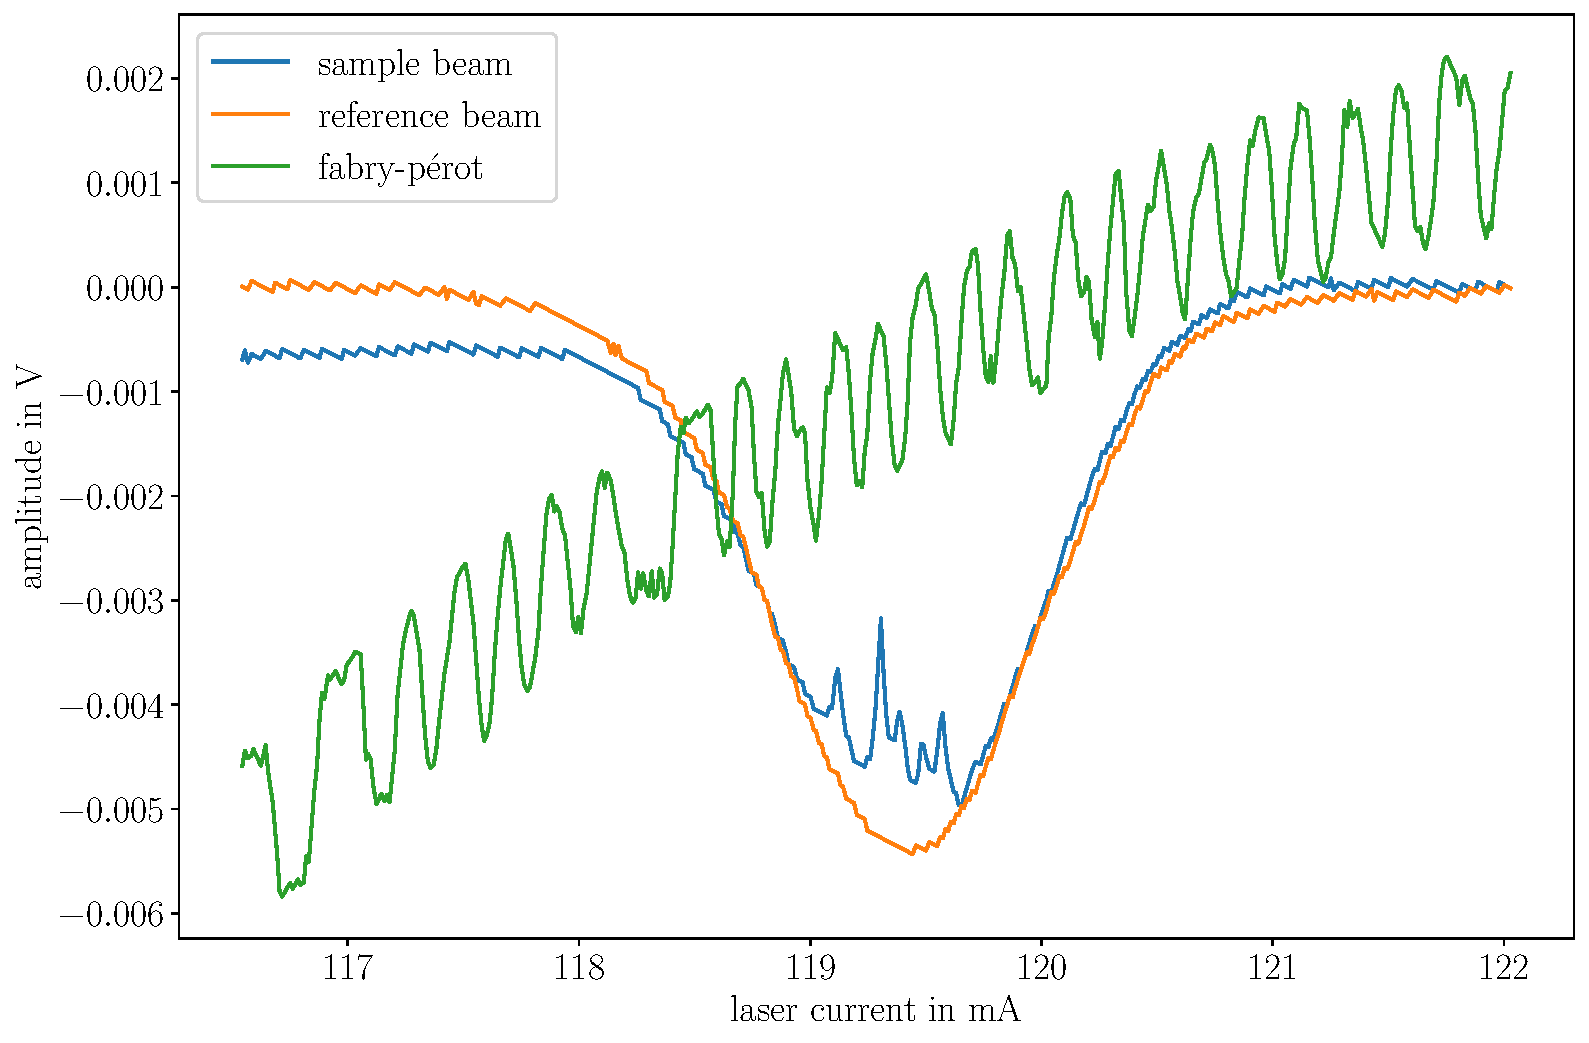
\includegraphics[scale=0.47]{Aufg-4/hyperfine1.pdf}
    \captionof{figure}{absorption spectrum of peak number 1}
    \label{image:peak1}
\end{center}
\begin{center}
    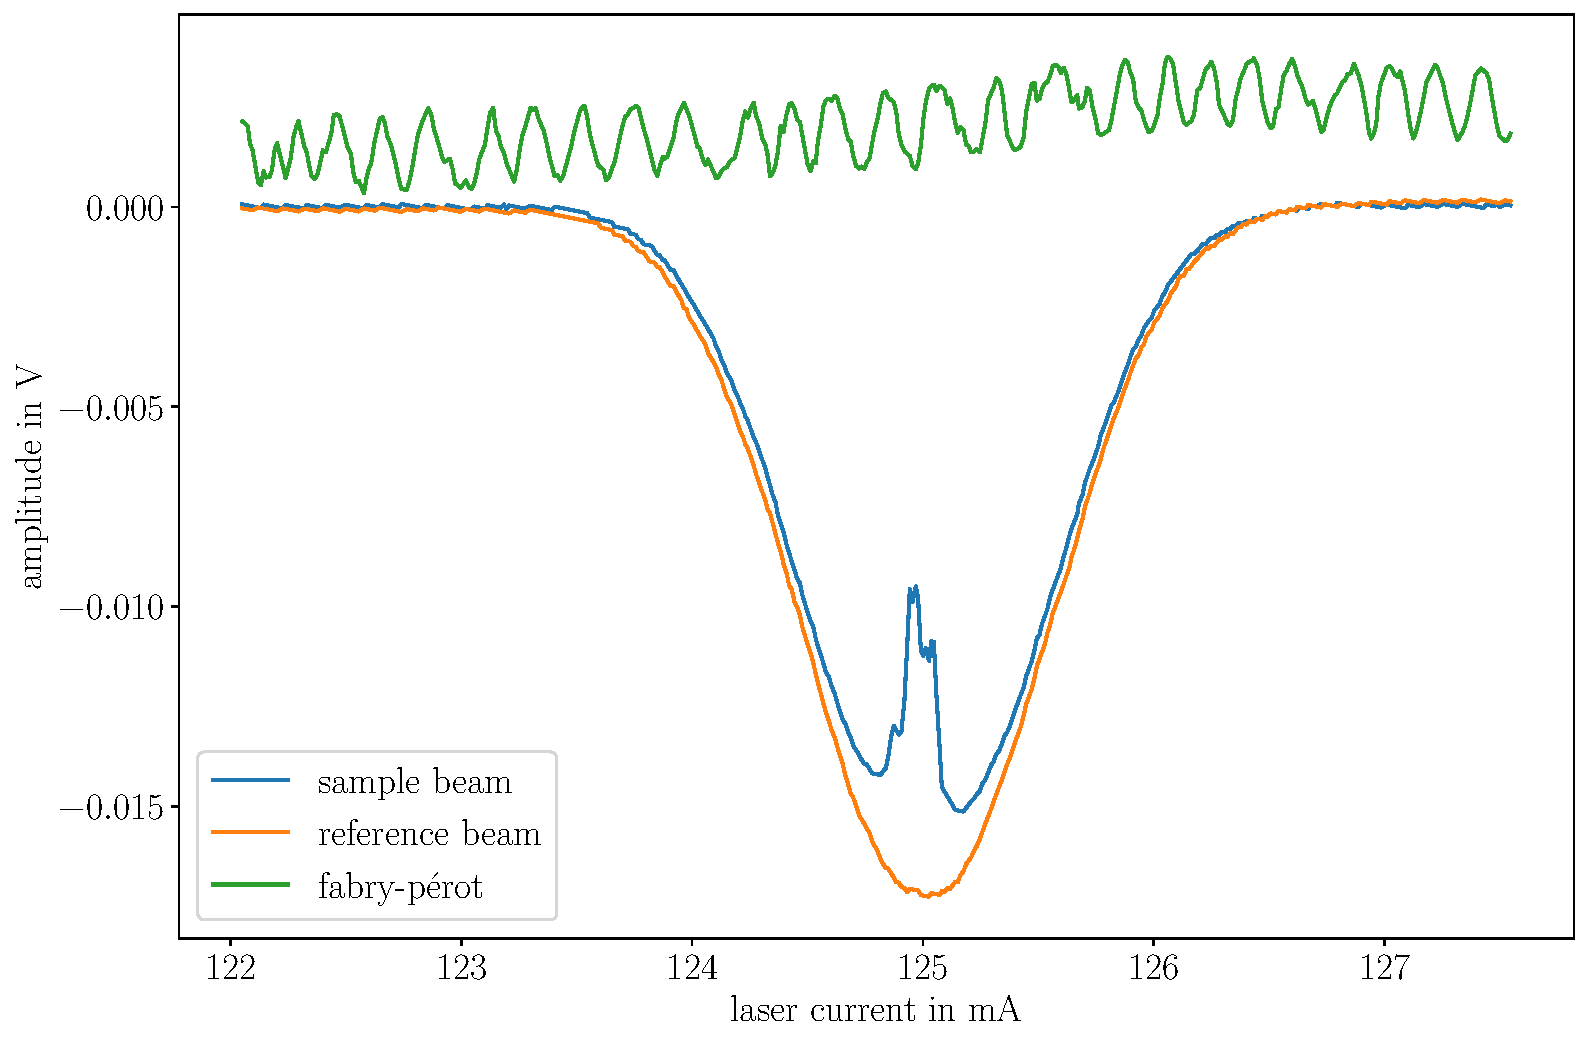
\includegraphics[scale=0.47]{Aufg-4/hyperfine2.pdf}
    \captionof{figure}{absorption spectrum of peak number 2}
    \label{image:peak2}
\end{center}
\begin{center}
    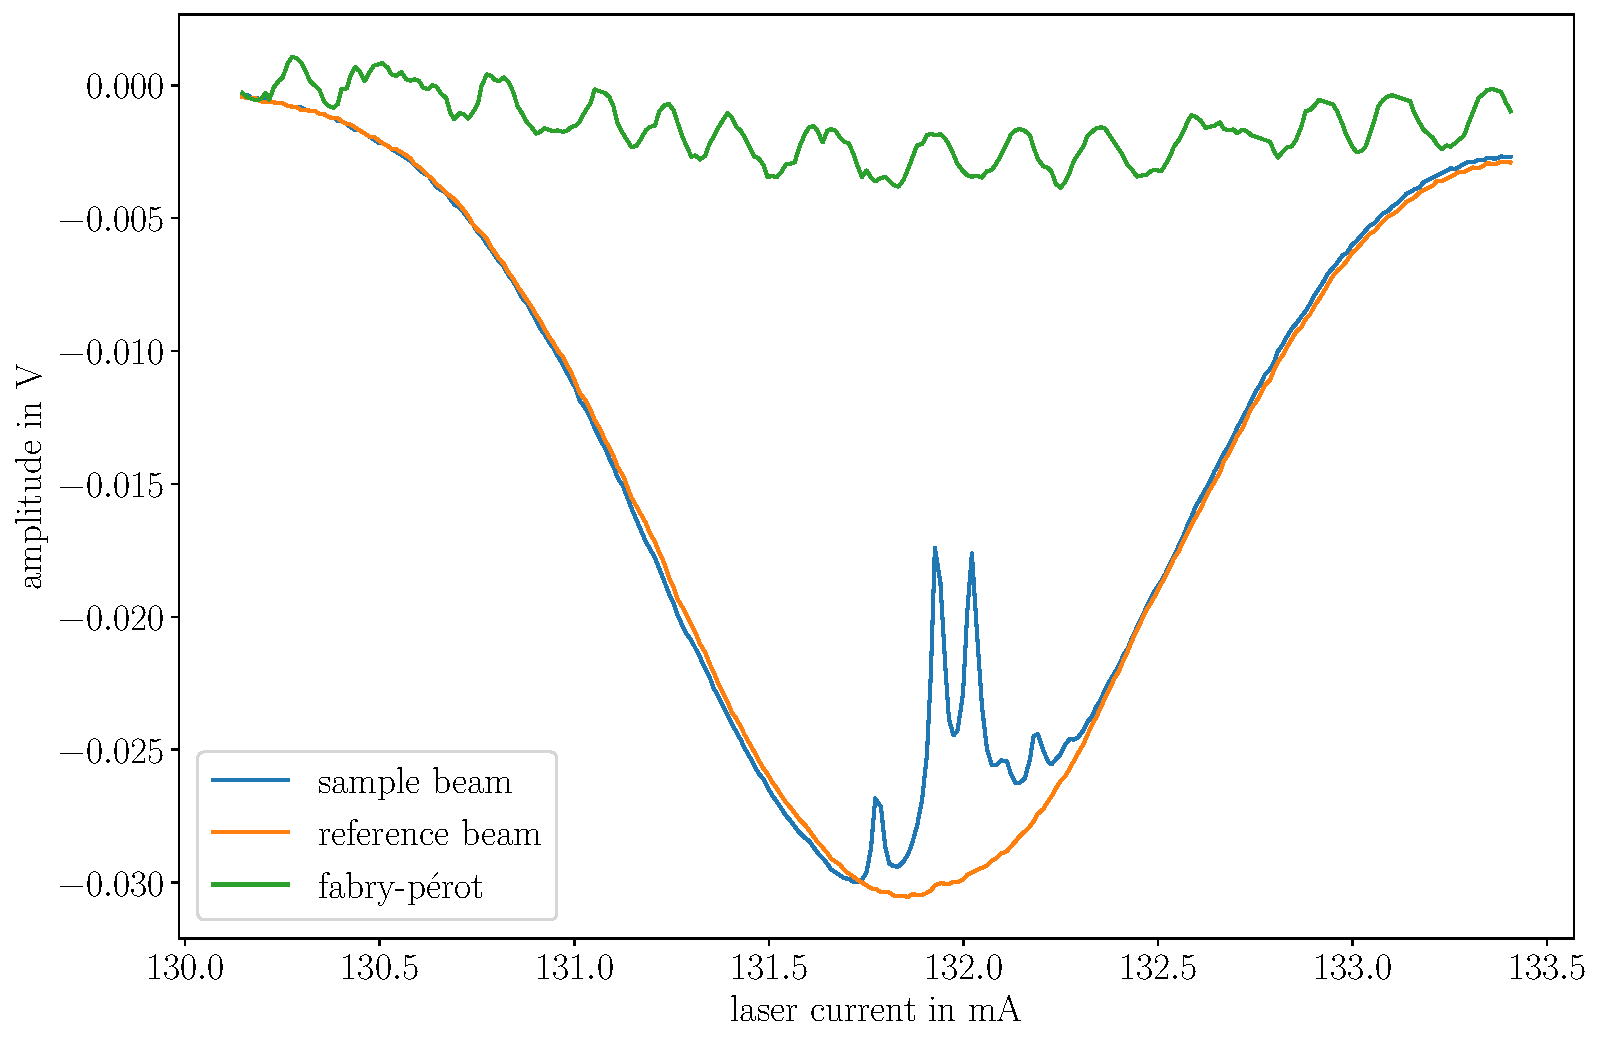
\includegraphics[scale=0.47]{Aufg-4/hyperfine3.pdf}
    \captionof{figure}{absorption spectrum of peak number 3}
    \label{image:peak3}
\end{center}
\begin{center}
    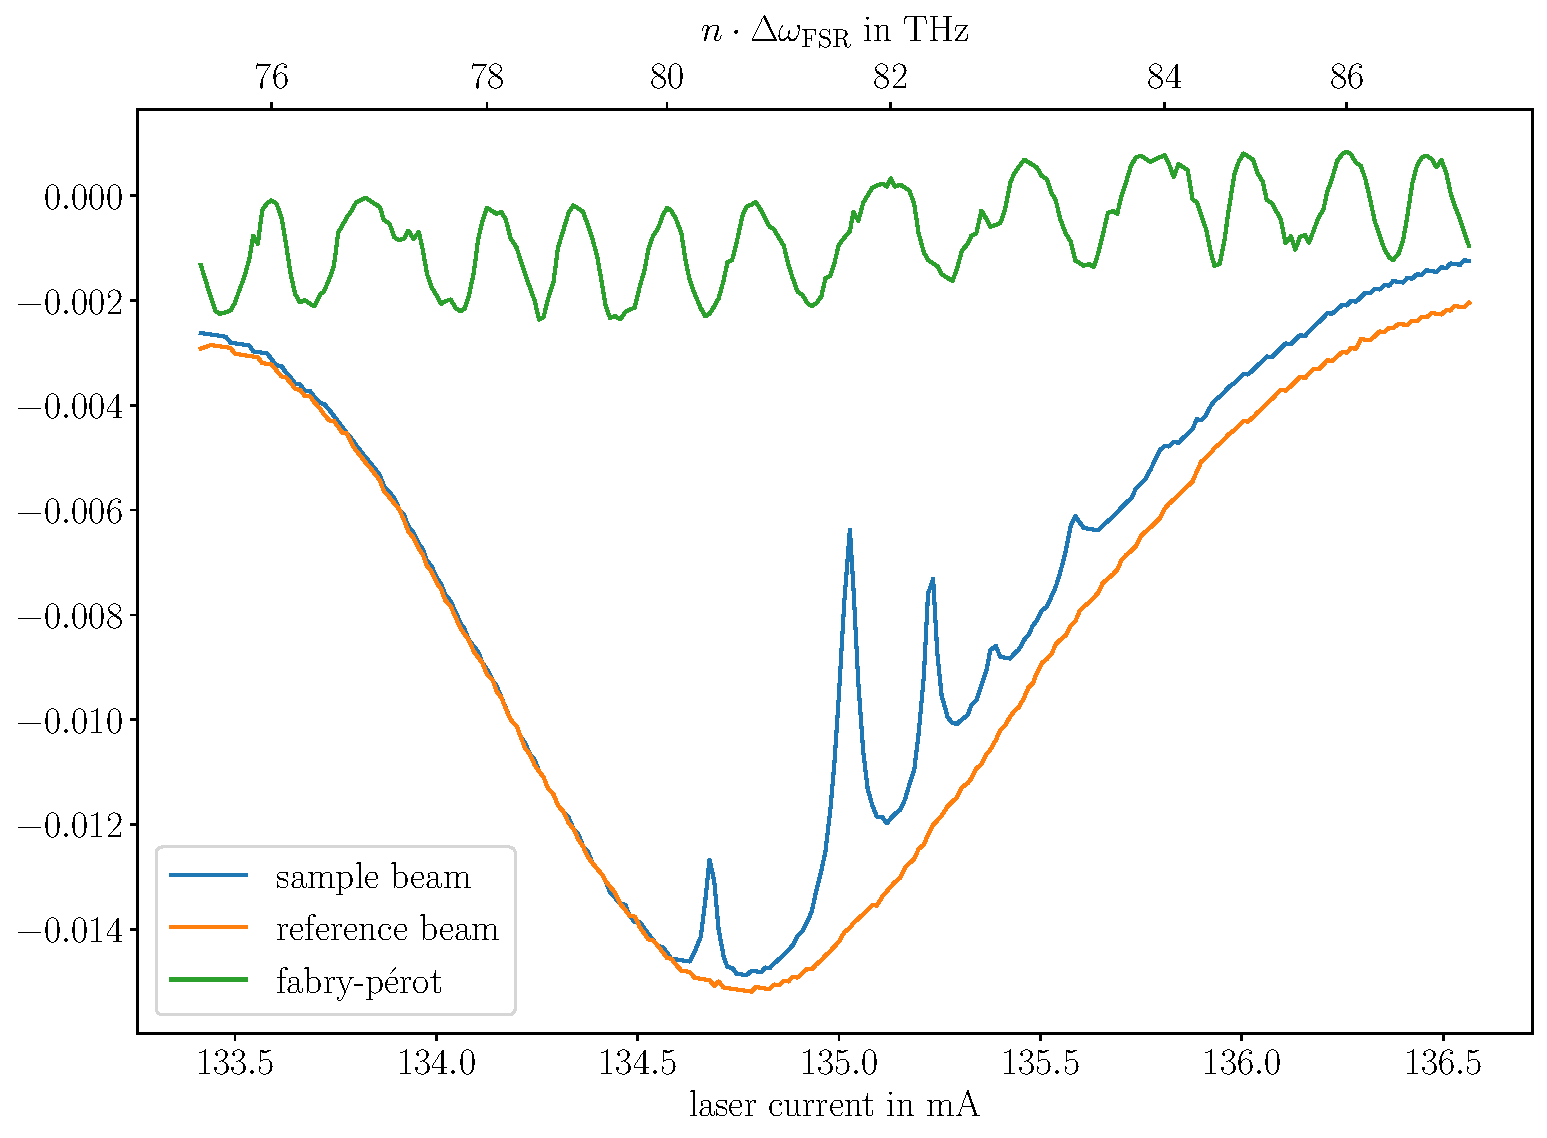
\includegraphics[scale=0.47]{Aufg-4/hyperfine4.pdf}
    \captionof{figure}{absorption spectrum of peak number 4}
    \label{image:peak4}
\end{center}
\newpage
It was chosen to use the peak number 3 because there are the hyperfine dips clearly visible.
